\documentclass[twocolumn]{aastex63}

\usepackage{graphicx}
\usepackage{amsmath}
\usepackage{natbib}

\shorttitle{Tidal Debris Forecast for Dwarf Galaxies}
\shortauthors{Li \& Claude}

\begin{document}

\title{Forecasting Tidal Debris Detection Around Milky Way and M31 Dwarf Satellite Galaxies for Next-Generation Spectroscopic Surveys}

\author{Ting S.\ Li}
\affiliation{Department of Astronomy \& Astrophysics, University of Toronto, Toronto, ON M5S 3H4, Canada}

\author{Claude}
\affiliation{Anthropic}

\begin{abstract}
We present a sensitivity study for detecting tidal debris around dwarf satellite galaxies of the Milky Way (MW) and M31 with next-generation spectroscopic surveys. For 65 MW and 40 M31 satellites drawn from the Local Volume Database, we estimate the number of observable stars in a tidal debris annulus between 5 and 20 half-light radii ($r_h$), assuming debris mass fractions $f = 0.001$--$1.0$ relative to the mass within $r_h$. We sample stellar populations from a Kroupa initial mass function, apply MIST isochrone photometry via \texttt{minimint}, and count stars brighter than $z$-band magnitude limits of 19, 21, and 23. At $f = 0.01$ and $z < 23$, the most promising MW targets include the LMC ($\sim7 \times 10^5$ stars), SMC ($\sim1.2 \times 10^5$), Sagittarius ($\sim4 \times 10^4$), and Fornax ($\sim1100$), while classical dwarfs like Draco and Sculptor yield $\sim$30--230 detectable stars. For M31, only the brightest satellites (M32, NGC~205, NGC~185) produce significant counts at this debris fraction. We compare these forecasts with debris fractions measured from $N$-body simulations of 922 satellite galaxies, finding a median $f_{5\text{-}20} \approx 0.02$ for satellites within 200~kpc of their host, consistent with our fiducial assumption. Approximately 45\% of simulated inner satellites have $f_{5\text{-}20} > 0.01$, suggesting that tidal debris at detectable levels is common. These results provide target lists and exposure requirements for upcoming wide-field spectroscopic facilities.
\end{abstract}

\keywords{dwarf galaxies --- tidal streams --- stellar surveys --- Local Group}

\section{Introduction} \label{sec:intro}

Dwarf satellite galaxies orbiting the Milky Way and M31 are subject to tidal forces that gradually strip stars from their outskirts. This tidal debris carries information about the satellite's orbit, mass loss history, and the gravitational potential of the host galaxy. Detecting and characterizing tidal features around dwarf galaxies is therefore a key science case for next-generation wide-field spectroscopic surveys.

While tidal tails and streams have been identified around several MW satellites---most notably Sagittarius \citep{Ibata1994, Majewski2003}, Tucana~III \citep{Drlica-Wagner2015}, and tentatively around others \citep{Munoz2006, Sand2009}---systematic searches for low-surface-brightness tidal debris in the outskirts of the full satellite population remain limited. Upcoming spectroscopic facilities with wide fields of view and deep limiting magnitudes will enable such searches, but planning requires quantitative forecasts of the expected signal.

In this work, we perform a comprehensive sensitivity study for 65 MW and 40 M31 dwarf satellite galaxies. We estimate the number of individually detectable stars in a tidal debris annulus spanning 5--20 half-light radii ($r_h$) as a function of the debris mass fraction $f$ and the survey depth (characterized by the $z$-band limiting magnitude). We further compare our assumed debris fractions with measurements from cosmological $N$-body simulations to assess how common detectable debris levels are in a $\Lambda$CDM context.

\section{Method} \label{sec:method}

\subsection{Satellite Sample} \label{sec:sample}

We draw satellite properties from the Local Volume Database \citep[LVDB;][]{Pace2024}. Our MW sample comprises 65 dwarf galaxies from the \texttt{dwarf\_mw} table, and our M31 sample includes 40 satellites from the \texttt{dwarf\_m31} table (hosted by either M31 or M33). For each satellite, we use the absolute $V$-band magnitude $M_V$, current stellar mass $M_\star$ (derived assuming a mass-to-light ratio $M/L = 2$), projected half-light radius $r_h$ (in physical units), heliocentric distance $d$, and spectroscopic metallicity [Fe/H] where available (defaulting to $-2.0$ otherwise).

\subsection{Debris Model} \label{sec:debris}

We assume the satellite's stellar mass follows a Plummer profile with scale radius equal to $r_h$. The projected mass enclosed within radius $R$ is:
\begin{equation}
    M(<R) = M_{\rm total} \frac{R^2}{R^2 + r_h^2}.
\end{equation}
The mass within $r_h$ is therefore $M_{\rm half} = M_\star / 2$, where $M_\star$ is the total (current) stellar mass.

We parameterize the tidal debris mass as a fraction $f$ of $M_{\rm half}$:
\begin{equation}
    M_{\rm debris} = f \times M_{\rm half} = f \times M_\star / 2,
\end{equation}
and distribute this mass uniformly over the annular area between $5\,r_h$ and $20\,r_h$:
\begin{equation}
    A_{\rm debris} = \pi \left[(20\,r_h)^2 - (5\,r_h)^2\right] = 375\,\pi\,r_h^2.
\end{equation}
We explore $f \in \{0.001, 0.01, 0.1, 1.0\}$, spanning scenarios from minimal to extreme tidal stripping.

\subsection{Stellar Population Synthesis} \label{sec:sps}

For each satellite, we generate a reference stellar cluster of $5 \times 10^4\,M_\odot$ using the Kroupa initial mass function \citep{Kroupa2001} via the \texttt{imf} package. We remove all stars with initial mass $> 1\,M_\odot$, as these have evolved off the main sequence after 12~Gyr. The surviving stellar mass $M_{\rm surv,ref}$ defines our scaling: for a given debris mass $M_{\rm debris}$, we scale the reference population by $M_{\rm debris} / M_{\rm surv,ref}$.

We compute apparent magnitudes in DECam $g$, $r$, $i$, $z$ and Bessell $V$ bands using the MIST isochrone interpolator \texttt{minimint} \citep{Choi2016}, evaluated at the satellite's metallicity and an age of 12~Gyr. The distance modulus $\mu = 5\log_{10}(d/\text{10\,pc})$ converts absolute to apparent magnitudes. We count stars with apparent $z < z_{\rm lim}$ for limiting magnitudes $z_{\rm lim} \in \{19, 21, 23\}$.

To reduce stochastic noise, we average results over 10 independent realizations of the reference cluster for each satellite.

\subsection{Stellar Mass--Size Relation} \label{sec:masssize}

For converting between stellar mass and half-light radius in the simulation comparison, we derive a relation from the observed $M_V$--size relation for Local Group dwarfs:
\begin{equation}
    \log_{10}(r_h / \text{pc}) = 0.31 \log_{10}(M_\star / M_\odot) + 0.49,
\end{equation}
assuming $M/L = 1.6$. This relation is validated against the LVDB data for both MW and M31 satellites (Figure~\ref{fig:masssize}).

\begin{figure}
    \centering
    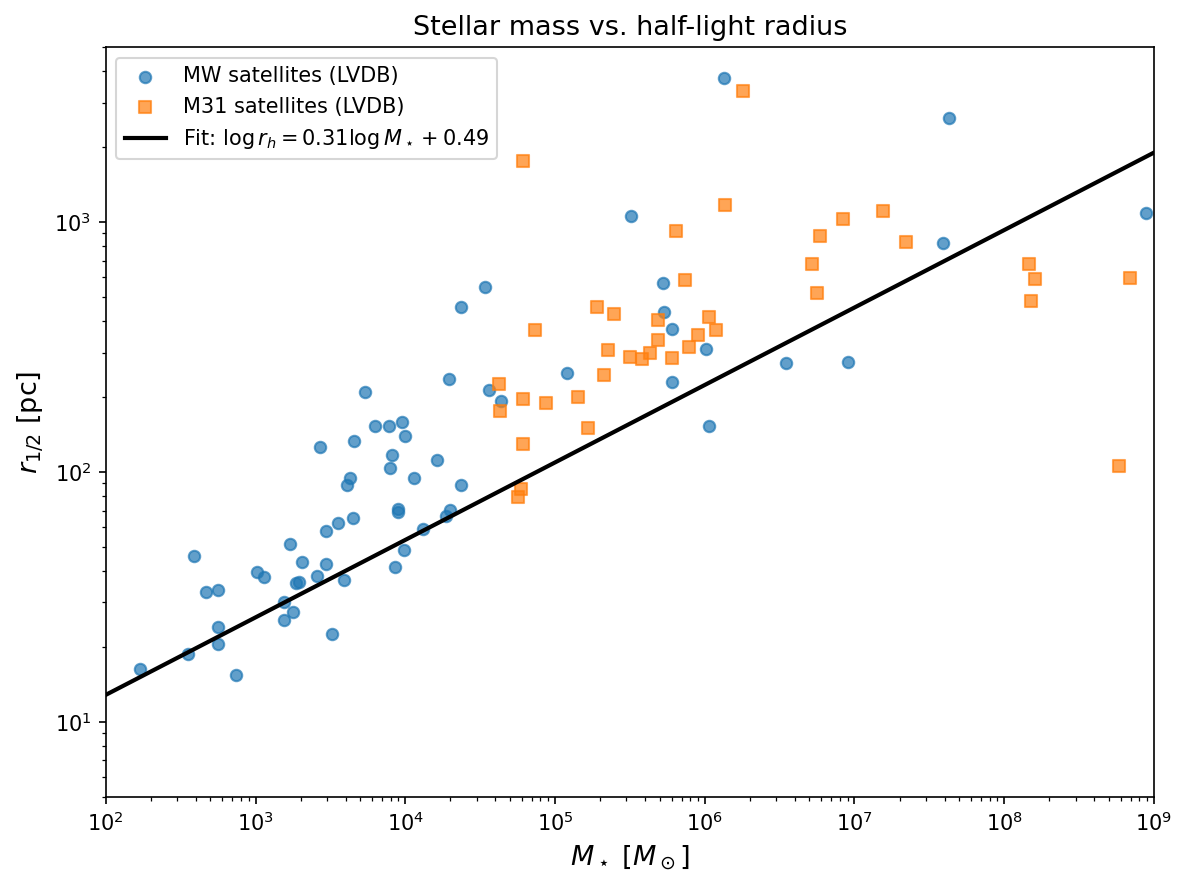
\includegraphics[width=\columnwidth]{mstar_rhalf_check.png}
    \caption{Stellar mass vs.\ half-light radius for MW (blue circles) and M31 (orange squares) satellites from LVDB, compared with the fitted relation $\log r_h = 0.31 \log M_\star + 0.49$ (black line).}
    \label{fig:masssize}
\end{figure}

\section{Results} \label{sec:results}

\subsection{Individual Satellite Forecasts} \label{sec:individual}

Figure~\ref{fig:draco} shows a representative example for Draco ($M_V = -8.9$, $M_\star = 10^{5.78}\,M_\odot$, $d = 81.5$~kpc, [Fe/H] $= -1.98$). The left panel shows the predicted number of detectable debris stars $N_{\rm rem}$ as a function of $z$-band limiting magnitude for four debris fractions. At $f = 0.01$ and $z < 23$, we predict $\sim$41 observable stars spread over 30.6~deg$^2$, yielding a surface density of 1.3~deg$^{-2}$. The middle panel shows the corresponding surface density, and the right panel displays a color--magnitude diagram of the debris population.

The detectability depends strongly on survey depth: the predicted counts increase by roughly an order of magnitude between $z < 21$ and $z < 23$, as the faint main-sequence turnoff stars at $\sim$12~Gyr become accessible.

\begin{figure*}
    \centering
    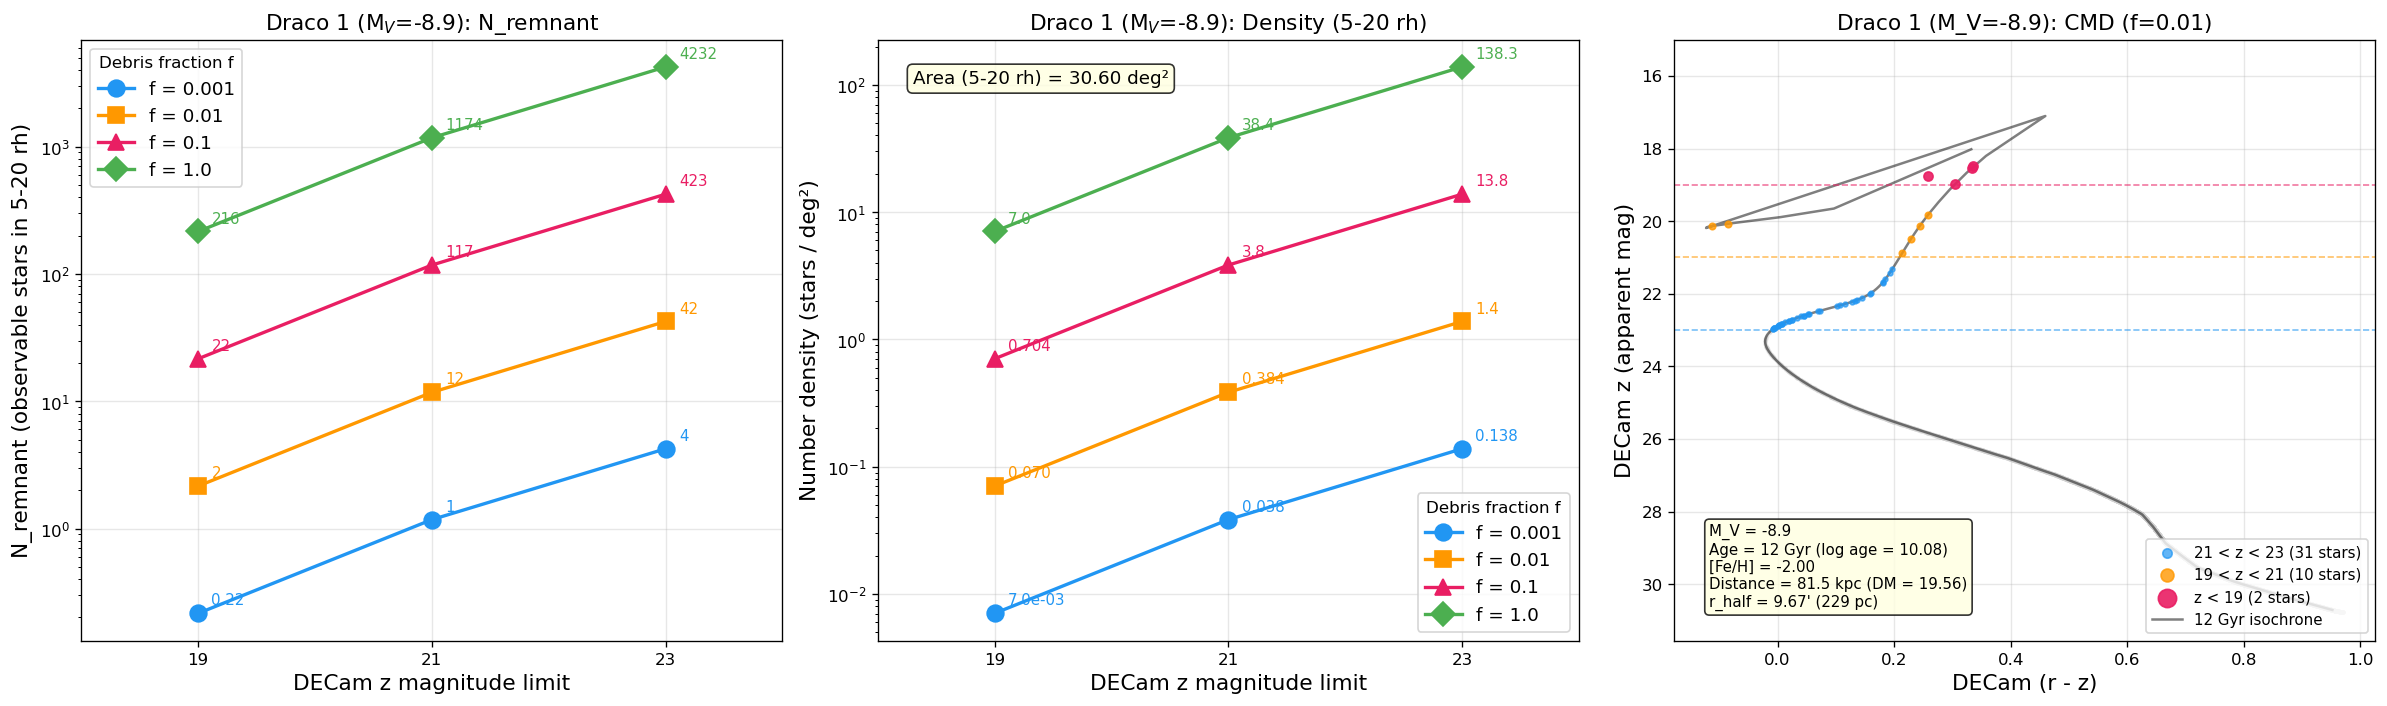
\includegraphics[width=\textwidth]{satellite_plots/mw/draco_1_debris.png}
    \caption{Tidal debris forecast for Draco. \textit{Left:} Number of detectable stars $N_{\rm rem}$ vs.\ $z$-band magnitude limit for debris fractions $f = 0.001$ (blue), 0.01 (orange), 0.1 (green), and 1.0 (red). \textit{Middle:} Surface density of debris stars. \textit{Right:} Color--magnitude diagram of the debris stellar population at $f = 0.01$, with the $z$-band limits indicated by horizontal lines.}
    \label{fig:draco}
\end{figure*}

\subsection{MW Satellite Summary} \label{sec:mw}

Figure~\ref{fig:mw_summary} presents the summary for all 65 MW satellites at our fiducial parameters ($f = 0.01$, $z < 23$). The top-left panel ranks satellites by predicted debris star count. The LMC ($\sim7.4 \times 10^5$), SMC ($\sim1.2 \times 10^5$), and Sagittarius ($\sim4.0 \times 10^4$) dominate, followed by Fornax ($\sim$1100), Sculptor ($\sim$230), and Leo~I ($\sim$150). Classical dwarfs such as Ursa Minor, Carina, and Draco each yield $\sim$40--65 stars.

The top-right panel shows $N_{\rm rem}$ vs.\ heliocentric distance, revealing the expected inverse trend: nearby satellites produce more detectable stars at fixed $f$. The bottom panels show correlations with $M_V$, demonstrating that both $N_{\rm rem}$ and the surface density scale strongly with luminosity. Ultra-faint dwarfs ($M_V \gtrsim -5$) generally produce fewer than one detectable star at $f = 0.01$.

\begin{figure*}
    \centering
    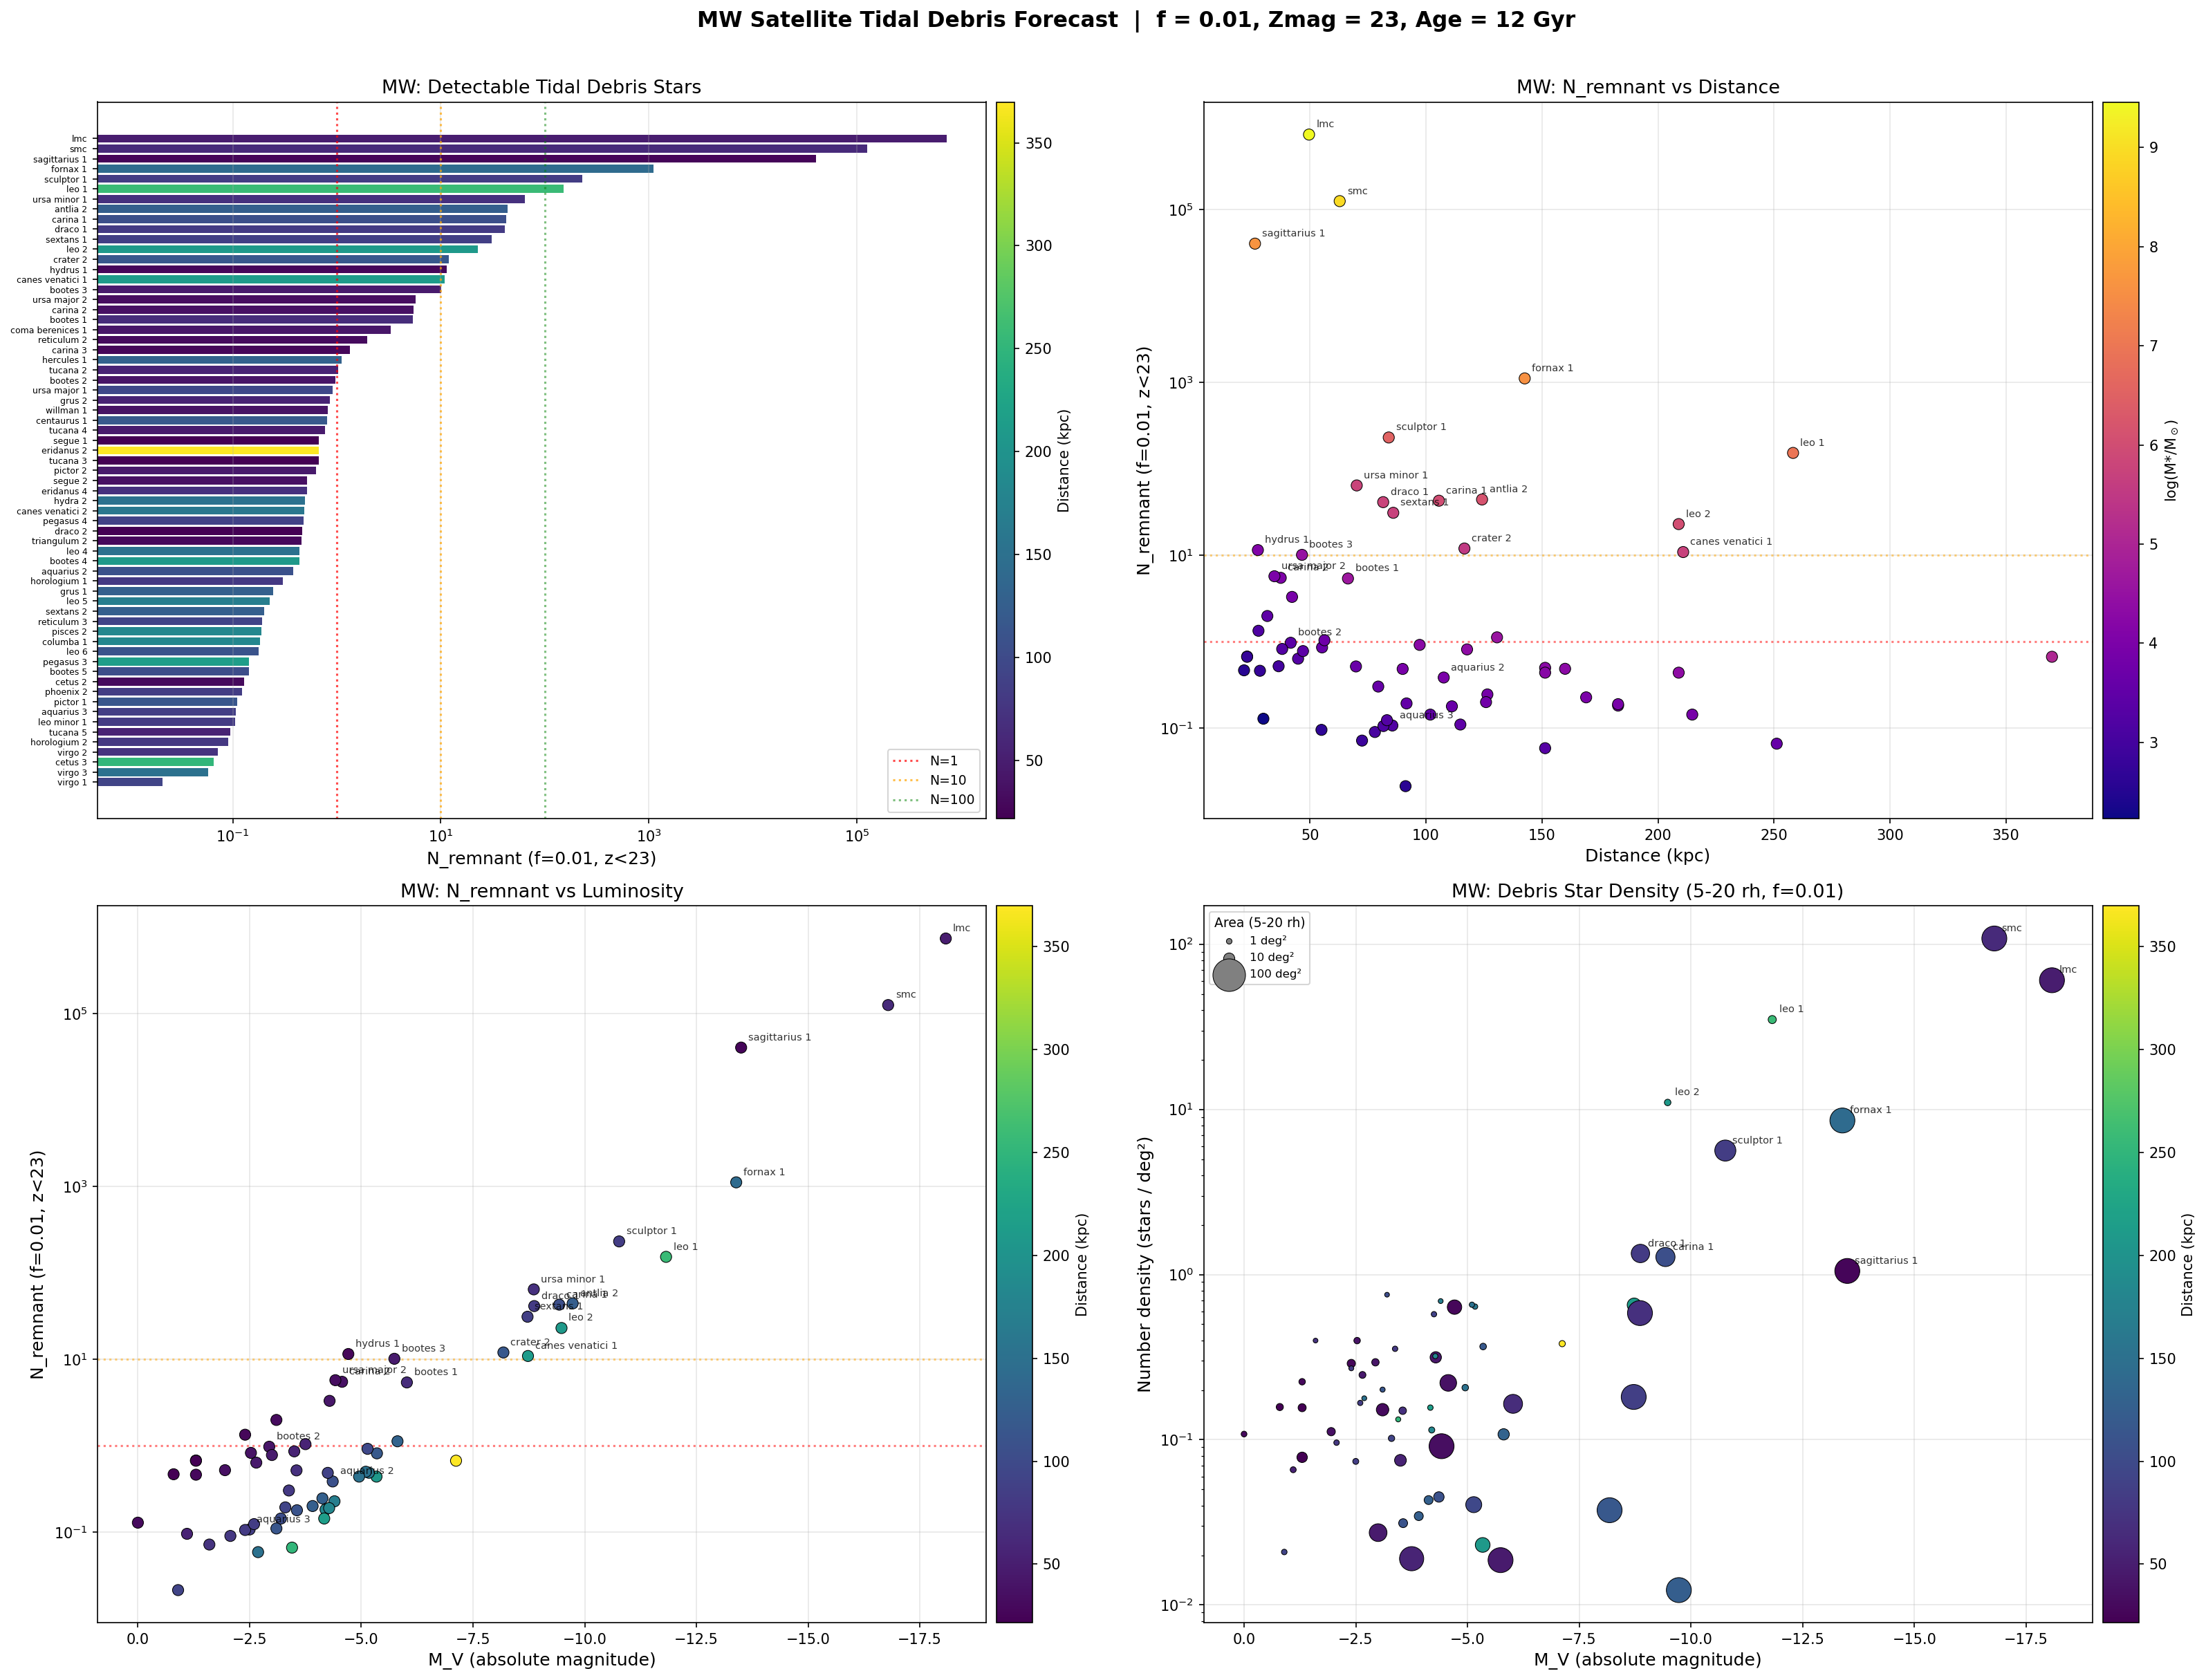
\includegraphics[width=\textwidth]{mw_satellites_debris.png}
    \caption{Summary of tidal debris forecasts for 65 MW satellites at $f = 0.01$ and $z < 23$. \textit{Top left:} Bar chart of $N_{\rm rem}$ ranked by count (top 20 shown). \textit{Top right:} $N_{\rm rem}$ vs.\ heliocentric distance. \textit{Bottom left:} $N_{\rm rem}$ vs.\ $M_V$. \textit{Bottom right:} Surface density vs.\ $M_V$.}
    \label{fig:mw_summary}
\end{figure*}

\subsection{M31 Satellite Summary} \label{sec:m31}

Figure~\ref{fig:m31_summary} shows the equivalent summary for 40 M31 satellites. Due to their $\sim$700--900~kpc distances, only the most massive satellites produce significant counts: M32 ($\sim$1060 stars, but extremely compact at $\sim$14,600~deg$^{-2}$), NGC~205 ($\sim$770), NGC~185 ($\sim$360), IC~10 ($\sim$240), and NGC~147 ($\sim$235). The classical M31 dwarfs (Andromeda~I through VII) yield 8--32 stars, while fainter satellites produce fewer than one detectable star at $f = 0.01$.

\begin{figure*}
    \centering
    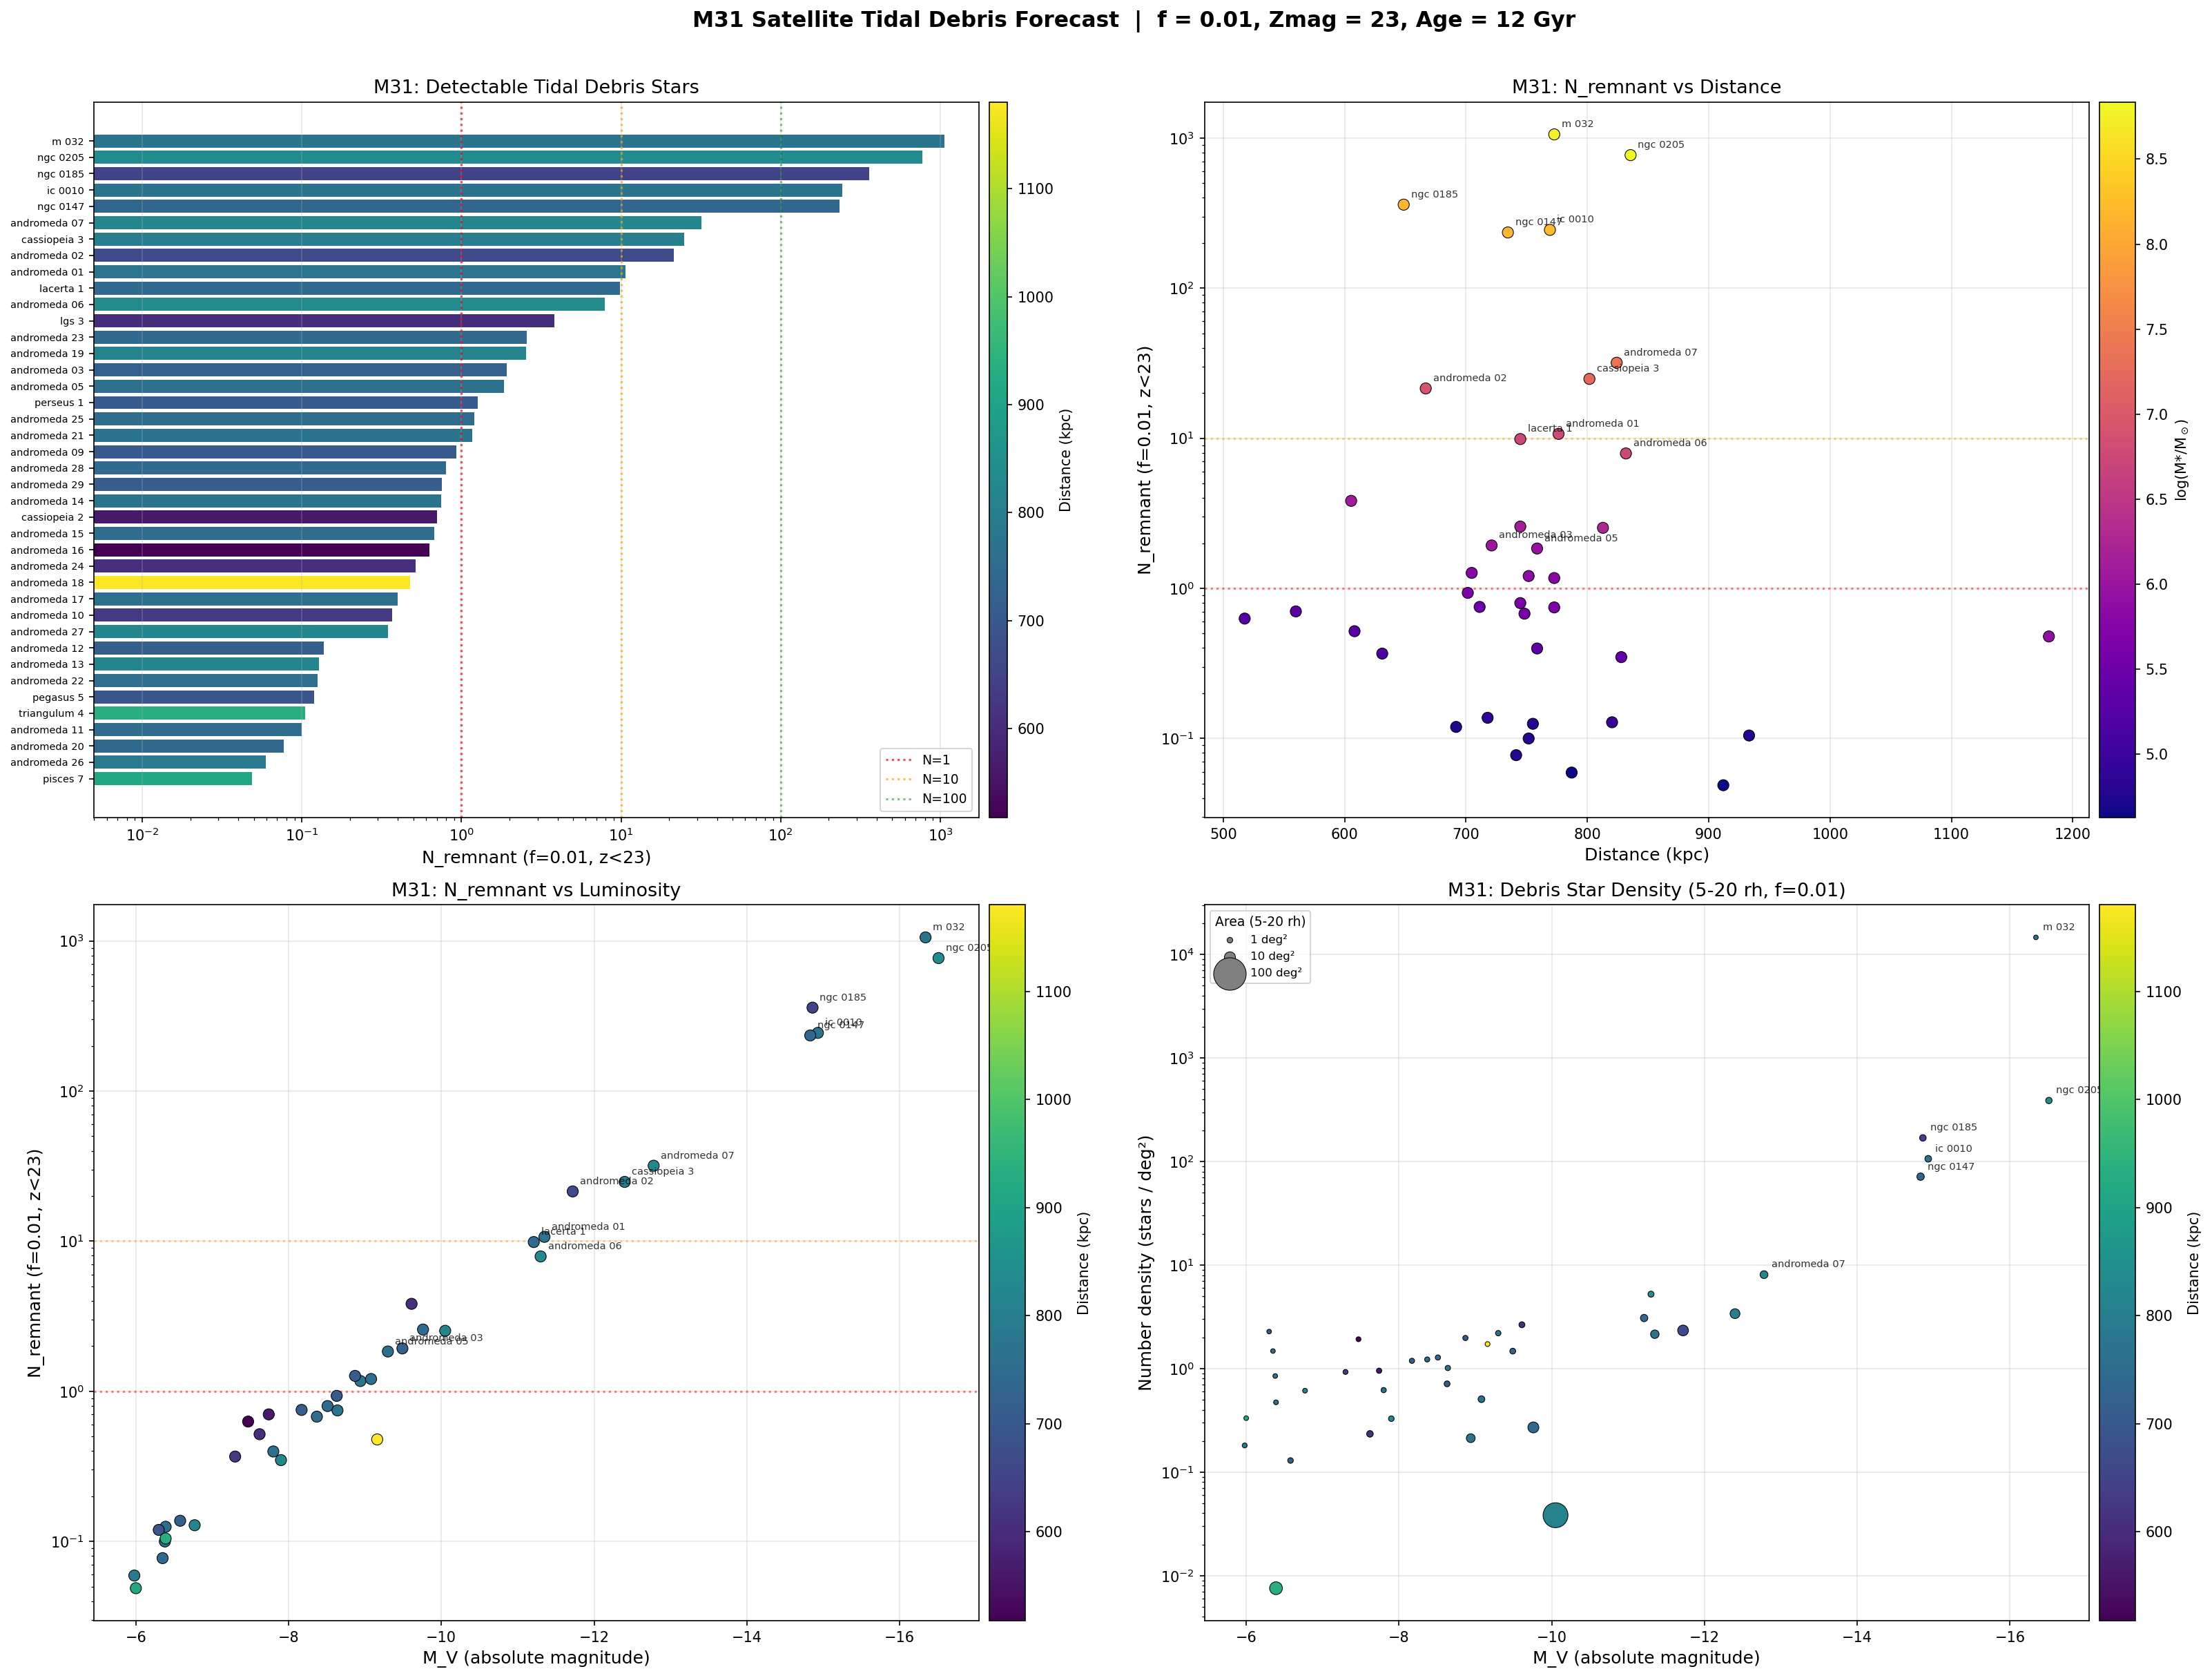
\includegraphics[width=\textwidth]{m31_satellites_debris.png}
    \caption{Same as Figure~\ref{fig:mw_summary} but for 40 M31 satellites.}
    \label{fig:m31_summary}
\end{figure*}

\section{Comparison with N-body Simulations} \label{sec:sims}

To assess how realistic our assumed debris fractions are, we compare with $N$-body simulation data from 922 satellite galaxies. For each simulated satellite, we compute the debris fraction as the ratio of stellar mass in the 5--20~$r_h$ annulus to mass within $r_h$:
\begin{equation}
    f_{5\text{-}20} = \frac{M_\star(5\text{--}20\,r_h)}{M_\star(<r_h)},
\end{equation}
using cumulative mass profiles measured from particle data.

Figure~\ref{fig:sim_fraction} shows $f_{5\text{-}20}$ as a function of six galaxy properties, color-coded by the bound stellar fraction $f_{\star,\rm bound}$. There is a strong correlation between stripping severity and debris fraction: intact satellites ($f_{\star,\rm bound} > 0.95$) have median $f_{5\text{-}20} \approx 0.002$, while heavily stripped systems ($f_{\star,\rm bound} < 0.5$) reach median $f_{5\text{-}20} \approx 0.4$. The tick marks along the top of each panel indicate where MW (blue) and M31 (orange) satellites fall in these property spaces.

\begin{figure*}
    \centering
    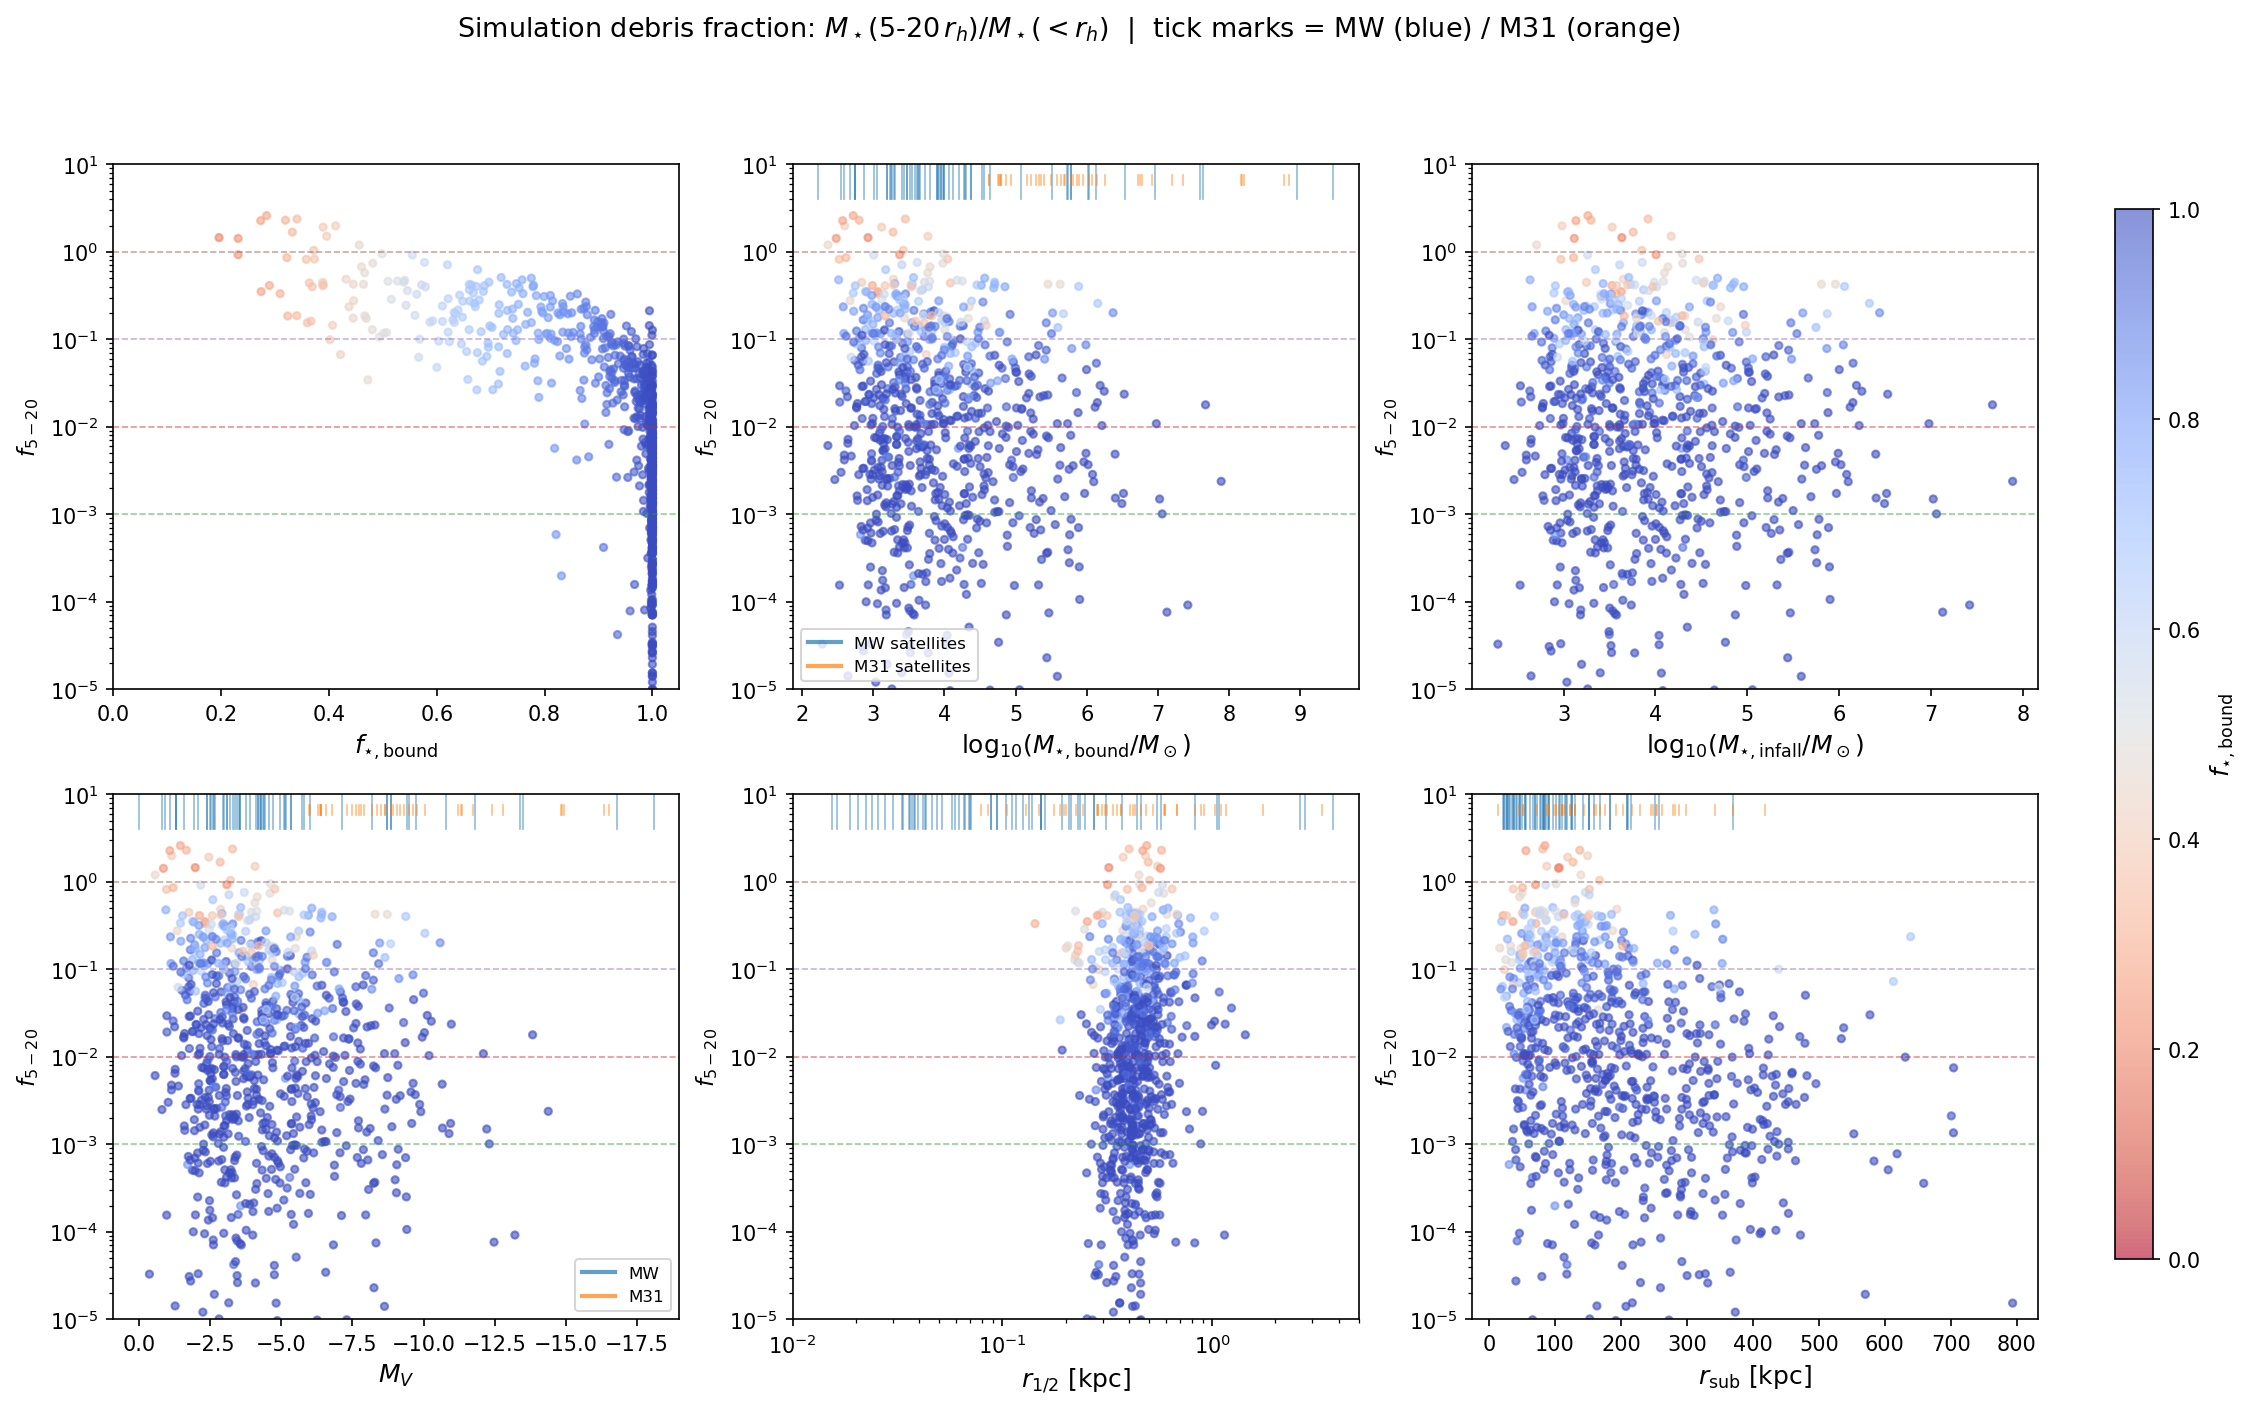
\includegraphics[width=\textwidth]{sim_debris_fraction_ticks.png}
    \caption{Debris fraction $f_{5\text{-}20}$ from $N$-body simulations vs.\ galaxy properties, color-coded by bound stellar fraction. Tick marks at the top of each panel show MW (blue) and M31 (orange) satellite values. Dashed horizontal lines mark $f = 0.001$, 0.01, 0.1, and 1.0. \textit{Top row:} $f_{\star,\rm bound}$, bound stellar mass, infall stellar mass. \textit{Bottom row:} $M_V$, half-light radius, distance from host.}
    \label{fig:sim_fraction}
\end{figure*}

Figure~\ref{fig:cumulative} shows the cumulative distribution of $f_{5\text{-}20}$. Restricting to satellites within 200~kpc of their host (comparable to the MW satellite population), the median debris fraction is $f_{5\text{-}20} \approx 0.022$, and approximately 45\% of satellites exceed our fiducial $f = 0.01$. The distribution does not reach unity at the low-$f$ end because $\sim$25\% of satellites have effectively zero debris ($f_{5\text{-}20} < 10^{-5}$, below the log-scale plot range).

\begin{figure}
    \centering
    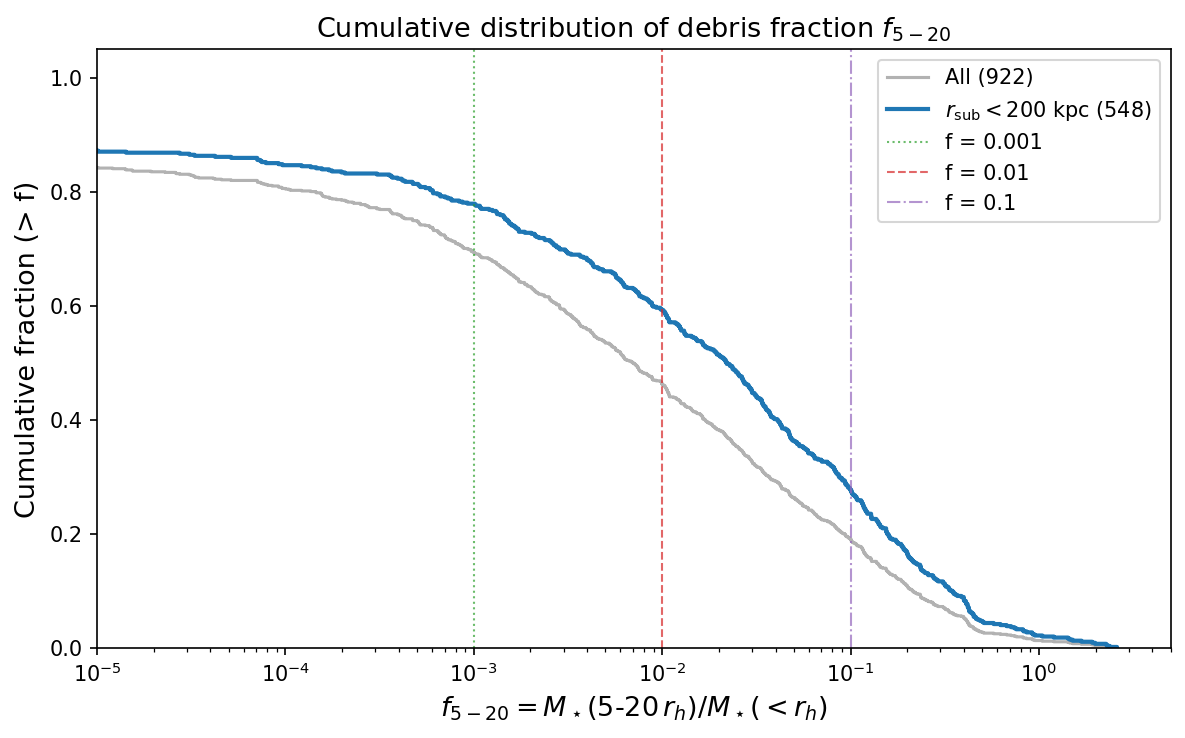
\includegraphics[width=\columnwidth]{sim_f520_cumulative.png}
    \caption{Cumulative fraction of simulated satellites with debris fraction exceeding a given $f_{5\text{-}20}$. The blue curve restricts to satellites within 200~kpc of the host ($N = 548$), while the grey curve shows the full sample ($N = 922$). Vertical lines mark reference debris fractions.}
    \label{fig:cumulative}
\end{figure}

Table~\ref{tab:sim_stats} summarizes the debris fraction statistics by stripping severity. These results suggest that a fiducial $f = 0.01$ is a reasonable lower bound for moderately stripped systems, while many satellites---particularly those on close orbits---may have significantly higher debris fractions.

\begin{deluxetable}{lccc}
\tablecaption{Debris Fraction Statistics by Stripping Level \label{tab:sim_stats}}
\tablewidth{0pt}
\tablehead{
    \colhead{Category} & \colhead{$N$} & \colhead{Median $f_{5\text{-}20}$} & \colhead{16--84\%}
}
\startdata
Intact ($f_{\rm bound} > 0.95$) & 653 & 0.002 & 0.000--0.019 \\
Mildly stripped (0.8--0.95) & 120 & 0.081 & 0.021--0.177 \\
Moderately stripped (0.5--0.8) & 103 & 0.200 & 0.071--0.418 \\
Heavily stripped ($< 0.5$) & 46 & 0.435 & 0.164--1.499 \\
\enddata
\end{deluxetable}

\section{Discussion} \label{sec:discussion}

\subsection{Target Prioritization}

Our results identify a natural hierarchy of targets for tidal debris searches. For the MW, the top-tier targets (LMC, SMC, Sagittarius) already have known tidal features and will yield enormous samples with next-generation surveys. The second tier---Fornax, Sculptor, Leo~I, and other classical dwarfs---represents the most scientifically valuable targets, as their debris fractions are less well constrained and the predicted counts ($\sim$40--1100 at $f = 0.01$) are within reach of deep spectroscopic surveys.

Ultra-faint dwarfs generally produce fewer than one detectable star at $f = 0.01$, consistent with their low stellar masses. However, a few nearby UFDs (Hydrus~1, Ursa Major~II, Carina~2) produce $\sim$5--11 stars, suggesting that deep targeted observations could probe their tidal status.

For M31, only the brightest satellites (M32, NGC~205, NGC~185, NGC~147, IC~10) are viable targets for individual star spectroscopy. Their compact angular sizes, however, mean that the debris surface densities can be very high (e.g., $\sim$14,600~deg$^{-2}$ for M32), potentially enabling detection in small survey footprints.

\subsection{Simulation Context}

The comparison with $N$-body simulations provides important context for interpreting our forecasts. The simulations show that (i) debris fractions span several orders of magnitude, from $< 10^{-5}$ for intact satellites to $> 1$ for heavily stripped systems; (ii) among inner satellites ($r_{\rm sub} < 200$~kpc), roughly half exceed $f = 0.01$; and (iii) the debris fraction correlates strongly with the bound fraction but shows no strong dependence on stellar mass or half-light radius at fixed stripping level.

These findings suggest that our fiducial $f = 0.01$ is conservative for the typical satellite, and that many systems---particularly those on close or eccentric orbits---may host substantially more debris.

\subsection{Caveats}

Several simplifications affect our predictions. We assume a single old (12~Gyr) stellar population, neglecting age and metallicity gradients that could affect the debris color--magnitude distribution. Our Plummer profile assumption may not accurately describe the mass distribution of all satellites, particularly irregular or tidally distorted systems. We do not model background contamination from MW foreground stars or unresolved galaxies, which will reduce the effective signal-to-noise ratio.

The IMF choice also introduces systematic uncertainty: using a Chabrier IMF instead of Kroupa yields $\sim$25\% more detectable stars at fixed debris mass, due to the different mass distributions near the hydrogen-burning limit.

\section{Summary} \label{sec:summary}

We have performed a comprehensive sensitivity study for detecting tidal debris around 65 MW and 40 M31 dwarf satellite galaxies. Our main findings are:

\begin{enumerate}
    \item At $f = 0.01$ and $z < 23$, classical MW dwarfs produce $\sim$30--1100 detectable debris stars in the 5--20~$r_h$ annulus, with surface densities of $\sim$0.2--9~deg$^{-2}$.
    \item For M31, only the five brightest satellites (M32, NGC~205, NGC~185, IC~10, NGC~147) yield significant counts ($>$200 stars) at this debris fraction.
    \item $N$-body simulations predict a median debris fraction $f_{5\text{-}20} \approx 0.02$ for inner satellites, with $\sim$45\% exceeding $f = 0.01$.
    \item Survey depth is critical: counts increase by roughly an order of magnitude between $z < 21$ and $z < 23$.
\end{enumerate}

These forecasts provide a quantitative basis for planning tidal debris searches with next-generation spectroscopic surveys.

\begin{acknowledgments}
This work made use of the Local Volume Database \citep{Pace2024}, the \texttt{minimint} isochrone interpolation package, and the \texttt{imf} package for stellar mass sampling. This report was produced with assistance from Claude (Anthropic).
\end{acknowledgments}

\bibliography{references}
\bibliographystyle{aasjournal}

\end{document}
